
\documentclass[a4paper,10pt]{scrartcl}

% [packages I understand]\
\usepackage{cite}

\usepackage[colorlinks={blue}]{hyperref}
\usepackage{acro}
% \usepackage[printonlyused,withpage]{acronym}

% Using this to deal with gantt chart
\usepackage{pgfgantt}
\usepackage{lscape}
\usepackage{afterpage}

% [packages I don't understand]
% \usepackage[style=numeric]{biblatex}
% \usepackage{natbib}
\usepackage{lmodern}
\usepackage[T1]{fontenc}
\usepackage[a4paper, total={14cm, 24cm}]{geometry}
\usepackage{textcomp}
\usepackage{gensymb}
\usepackage{graphicx}
\usepackage{float}
\usepackage{caption}
\usepackage{paralist}
\usepackage{xcolor}
\usepackage{subcaption}
\usepackage[font={footnotesize,it}]{caption}
\usepackage{amsmath,amssymb,amsthm} 
\usepackage{url}
\usepackage{xspace}
\usepackage{algorithmic}
\usepackage{mathpazo}
\usepackage{booktabs}
\usepackage{subfiles}
\usepackage{silence}
\usepackage{listings}
\usepackage{verbatim}

% [Settings]

\WarningFilter{DuplicateLabels}

\newcommand{\ie}{ie}
\newcommand{\eg}{eg}
\newcommand{\reffig}[1]{Figure~\ref{#1}}
\newcommand{\refsec}[1]{Section~\ref{#1}}

\setcapindent{1em} %-- for captions of Figures
\setlength\parskip{1em plus 0.1em minus 0.2em}
\setlength\parindent{0pt}
\sffamily

\renewcommand{\algorithmicrequire}{\textbf{Input:}}
\renewcommand{\algorithmicensure}{\textbf{Output:}}

% \addbibresource{lib.bib}
% [Title Page] (could be split away)

\titlehead{\centering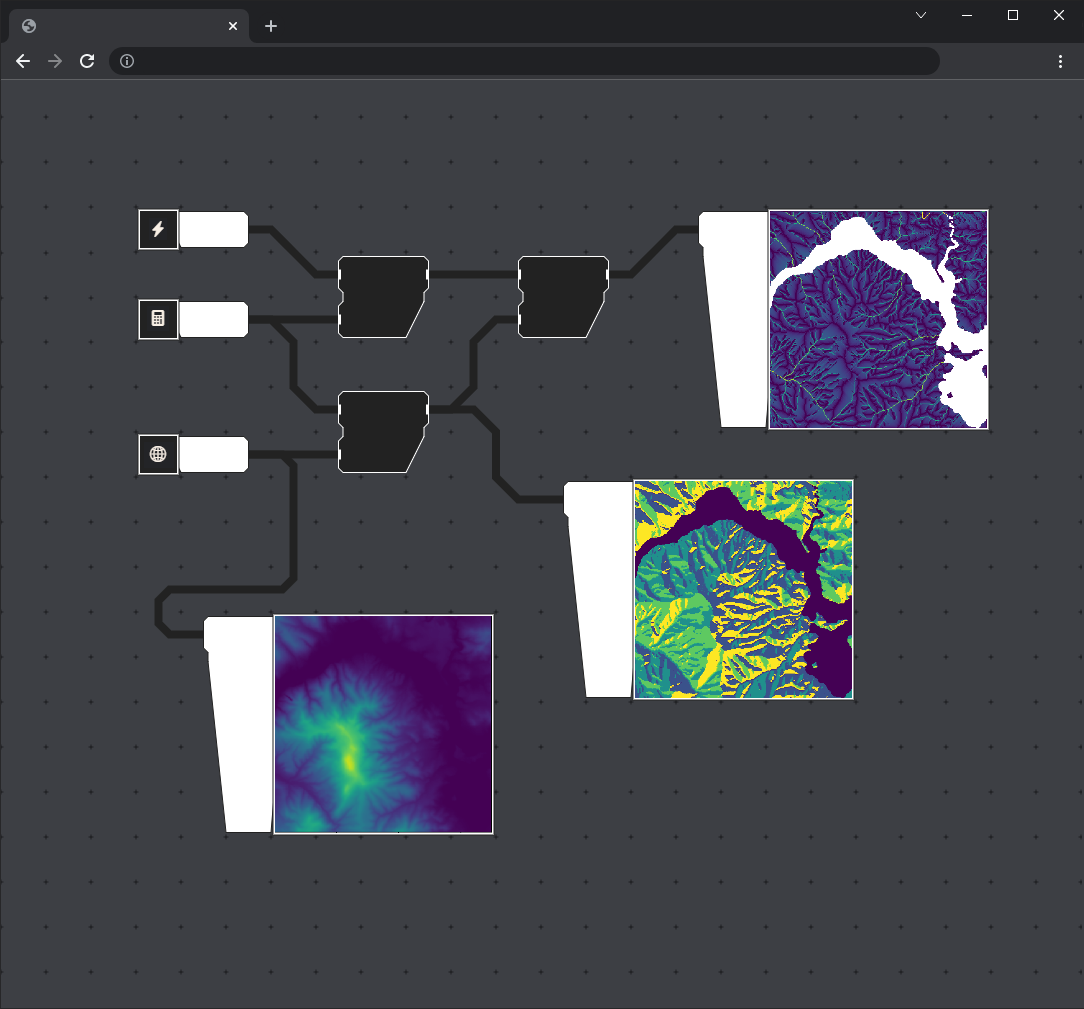
\includegraphics[width=12cm]{images/cool-image-4.png}}
\title{Thesis Proposal: \\
% Client-Side Geoprocessing using WebAssembly and Visual Programming
Accessible geoprocessing in a browser using WebAssembly and Visual Programming
% FAIR Geoprocessing: 
% Using WebAssembly to perform Geoprocessing directly in the browser.
}

\author{
  Jos Feenstra\\
  MSc Geomatics | TU Delft\\
  \#4465768 | \url{me@josfeenstra.nl}\\
  \\
  1st supervisor: Stelios Vitalis \\
  2nd supervisor: Ken Arroyo Ohori \\
}

\date{January, 2022}

% load acronyms before starting
\DeclareAcronym{w3c}{short=W3C, long=World Wide Web Consortium}
\DeclareAcronym{wasm}{short=Wasm, long=WebAssembly}
\DeclareAcronym{ux}{short=UX, long=User Experience}
\DeclareAcronym{vpl}{short=VPL, long=Visual Programming Language}
\DeclareAcronym{gui}{short=GUI, long=Graphical User Interface}


\begin{document}
  
\clearpage\maketitle
\thispagestyle{empty}
\sffamily

\begin{center}
  \textbf{Key words:} Geomatics, WebAssembly, 3D geometry, Geo processing, Client side, Visual programming, 
\end{center}

\newpage
\printacronyms

\newpage
\tableofcontents

\newpage
%-------------------------------------------------------------------------------------------------%
% An introduction in which the relevance of the project and its place in the 
% context of geomatics is described, along with a clearly-defined problem statement.
% [KEN]
% instead, I think you can start by saying that web applications are popular
% explain the benefits briefly
% apart from having no installation

% then, I think you can make a better argument for your thesis overall
% explain that historically, thin client fat server was the standard
% for the reasons you listed
% and then directly explain why this is potentially changing now

\newpage
\section{Introduction}

% Dissolving the discrepancy between visualization \& processing in web-apps.

% web is popular 
% geoweb-applications are popular 
% online geodata processing is popular 
% client-side geodata processing 


% STELIOS: Relatively slow
 
% show an example 

Interactive, browser-based \ac{gis} applications form an indispensable component of the modern geospatial software landscape. A web application is cross-platform in nature, and offers ease of maintainability and access, since no installment or app-store interaction is required to update or run the app. The ability be placed as a supplement within the larger context of a webpage is also not trivial. These features have made the browser a popular host for many \ac{gis} applications, especially when targeting end-users. 

% streamline these three paragraphs.
% I want something like -> problem: limitations. 

Despite the popularity of \ac{gis} web applications, the range of actual \ac{gis} abilities these applications are capable of is very limited. For example, \ac{geoprocessing}, like CRS translations, interpolation, boolean operations, or raster transformation kernels are usually not present within the same software environment as the web app. This limited range of capabilities limits the usefulness of \ac{gis} web applications, and with it the number of use cases a \ac{gis} web application can serve. Current geospatial web applications serve for the most part only as lightweight viewers; visualizers of pre-processed data. If web applications gain these functionalities, they could grow to be just as diverse and useful as desktop \ac{gis} applications. It would allow for a new range of interactive web applications, in which data users can post-process geodata quickly, uniquely, and on demand.

This raises the question of Why. Why are web \ac{gis} applications limited to just be viewers?

% This raises the question: why is this not done yet? two reasons 
% 1. People are content with server-side geoprocessing 
%    -> BUT: this does not serve every use-case 
% 2. Client-side geoprocessing is hindered by javascript and the web environment
%    -> NOT ANYMORE: WebAssembly
% 
% 
% To solve 2: WebAssembly
% To solve 1: We offer a case study which demonstrates a unique type of application which would not be possible without client-side geoprocessing. 

However, by making the functionality of an application not self-contained but distributed, 

The improvements of client-side hardware have opened up a second possibility: client-side geoprocessing, directly within a web application. By doing this, the hard divide between client visualization and server processing could be bridged.  while at the same time driving down the operational costs of geoprocessing servers. This is why client-side \ac{geoprocessing} in web applications is slowly gaining traction during the last decade \cite{kulawiak_analysis_2019, panidi_hybrid_2015, hamilton_client-side_2014}. 

% Interactive geospatial data manipulation and online geospatial data processing techniques are described as "current highly valuable trends in evolution of the Web mapping and Web GIS" \cite{panidi_hybrid_2015}. 

However, serious drawbacks to client-side geoprocessing where encountered during these studies. Browser-based geoprocessing suffers from the fact that it will need to be written in the `JavaScript` programming language. Previous attempts at client-side geoprocessing have shown that JavaScript based geoprocessing libraries do not offer the performance required for proper geodata processing \cite{hamilton_client-side_2014}. 
Moreover, the JavaScript library ecosystem does not offer viable alternatives to industry-standard libraries like CGAL and GDAL. 
% This would require alternatives to be rewritten in JavaScript, or would require the source code of mature libraries to be compiled to JavaScript. Both these solutions would be difficult to maintain, and would still end 
% Both these solutions contain many imperfections. The first option would be an inefficient, time-consuming task, and would mean code duplication. 
% The second option would mean taking C++-based libraries such as CGAL, and compiling them to a special, fast subset of JavaScript called `asm.js` using the `emscripten` compiler \cite{zakai_emscripten_2011}. 
% While this is more fast and reliable, it contains its own set of problems. 
% The generated, rather large JavaScript files usually take a long time to download, to scan, and to be properly optimized by a JavaScript Just In Time (JIT) Compiler \cite{haas_bringing_2017}. 

An emergent technology poses a solution to both problems. At the end of 2019, the \ac{w3c} officially pronounced WebAssembly as the fourth programming language of the web \cite{w3c_world_2019}. Since then, all major browsers have added official WebAssembly support. \ac{wasm} is a binary compilation target meant to be small, fast, containerized, and platform \& source independent \cite{haas_bringing_2017}. \ac{wasm} surpasses javascript in almost all performance aspects: it loads quicker, it is scanned quicker, and since it is close to bytecode, it can often run at a speed comparable to system level programming languages like C++ and Rust \cite{jangda_not_2019}. 

% \cite{beilschmidt_vat_2017}


% Related studies concerned with the performance of WebAssembly, together with the existing software around WebAssembly, pose enough evidence to suggest  theoretically possible (SOURCE: Emscriptem). 
% However, this leaves the question whether it is practically possible unanswered, evident by the fact that no wasm-powered geoprocessing tools exists at the time of writing this study. 

\newpage

% stelios: Speed up 

\subsection{Problem}

If WebAssembly performs as described by \cite{haas_bringing_2017} and \cite{jangda_not_2019}, it could theoretically be the missing link to make client-side geoprocessing viable. However, no wasm-powered geoprocessing tools exists yet at the time of writing. Hypothetically, this is because of two reasons. Firstly, WebAssembly brings along many practical uncertainties:

\begin{itemize}
  \item Do geoprocessing libraries directly compile into WebAssembly? If not, which workarounds are needed? 
  \item Will a \ac{wagl} load efficiently, or should they be split up into parts, and loaded lazily? 
  \item How well do \ac{wagl} operations perform in a browser, compared to their native counterparts? What can be done to make this difference as small as possible?
\end{itemize}

Secondly, the way geoprocessing is supposed to be performed within the context of a web-browser remains unknown. The above list of implementation considerations cover only how \ac{wagl}'s can be \emph{run}. Potential answers do not indicate how \ac{wagl}'s can be \emph{used}. \cite{jangda_not_2019} warns against assessing WebAssembly in a vacuum, and notes how its performance is highly dependent on the way it is used, and the context in which it is used. This context of geoprocessing within a web-browser brings up many considerations as well: 

\begin{itemize}
  \item How will users upload or specify the input in a web-browser?
  \item Can the transformations offered by \ac{wagl}'s be used like functions? Or do they require special services, such as a wrapper library, virtual file system, or a virtual Command line interface? 
  \item How can users recieve and evaluate the output in a web-browser?
  \item How can a sequence of geoprocessing steps be chained together in a web-browser?
  \item How can a web-based \ac{ui} or \ac{gui} facilitate all these functionalities?
\end{itemize}

These two sets of unknowns are highly dependent upon each other. Together, they form a barrier preventing further development of client-side geoprocessing. Since no wasm-powered, client-side geoprocessing application exist yet, there is no way to answer these questions, and no way to confirm the theoretical benefits of WebAssembly for client-side geoprocessing, and the geospatial community at large.



\subsection{Use Case}
% mini methodolody??


in order to demonstrate 

visual programming language.




%-------------------------------------------------------------------------------------------------%
\newpage

%-------------------------------------------------------------------------------------------------%
\subsection{Research Questions}

This study intends to discover if contemporary web technologies can facilitate client-side geoprocessing by seeking an answer to the following question:  

\textit{How to \textbf{design and create} a browser-based GIS environment which can \textbf{effectively utilize} \textbf{existing geoprocessing libraries}, using only the \textbf{current state} of \textbf{standard client-side web technologies}?}

\subsubsection*{Explanation}

% The research question is written purposefully written in the "how well does X support Y question" shape. To unpack its components: 

- \textbf{design and create}: The wording 'design and create' is used to signal that this will consider the theoretical design , as well as the practicalities of creating this design. 

- \textbf{Standard client-side web technologies}: This phrase is meant to limit the scope to only the standard, core technologies of major browsers (Chrome, Edge, Safari, Firefox). This means the four languages \ac{wasm}, CSS, JavaScript and HTML. Additionally, HTML5 gives us WebGl, the 2d Canvas API, SVG's, and Web Components to work with.

- \textbf{Current state}: The study will use contemporary, even bleeding edge features of the modern web, but its findings will nonetheless be bound to this time of writing, as web technologies in particular quickly change. 

- \textbf{Existing geoprocessing libraries}. This wording expresses this studies desire to explore the usage of existing geoprocessing libraries, rather than to recreate geoprocessing libraries from scratch.

- \textbf{Effectively utilize}: The study intends to not only find out how \ac{wagl}'s can be \textit{run} in a browser, but also how \ac{wagl}'s can be \textit{used}. 


\subsubsection*{Sub Questions}

The following sub-research questions are needed in order to answer the main question. The methodology chapter will explain the choices of these sub-questions. 

\textit{1 : What is the most fitting methodology of compiling C++ geoprocessing libraries to WebAssembly?}

\textit{2 : How to design and create a client-side geoprocessing interface for data-users?}

\textit{3 : How can wasm-compiled geoprocessing libraries be distributed and used in a client-side geoprocessing interface?}

\textit{4 : What are the advantages and disadvantages of GIS applications created using a client-side geoprocessing environment powered by WebAssembly?}

\newpage
\subsubsection*{Assessment}

At the final conclusion of the proposed thesis, we can answer if the designed and created GIS environment can indeed effectively utilize these geo-libraries.
this will be answered by quantitative and qualitative means:

Quantity
\begin{itemize}
    \item Have all required features been implemented?
    \item Which libraries can be used?
    \item What are the load \& run times of these libraries, compared to native execution?
\end{itemize} 

Quality
\begin{itemize}
    \item Have all design goals been met?
    \item Can data users 'effectively' handle input, process and output?
    \item Can the load \& run times be regarded as acceptable to use? 
\end{itemize} 


% ----
\subsection{Scope}


\subsection*{Will Include}

The 'will include' scope is represented by the Methodology chapter. 

%-----------------------------------------------------------------------------%
\subsection*{Will not include}

\subsubsection*{Server-side or Native WebAssembly} % **Client-side WebAssembly Only**

This study will limit itself to the \emph{client-side} usage of WebAssembly. 
A powerful case can be made for \emph{server-side}, or native level usage of WebAssembly, especially in conjunction with a programming language such as Rust. 
Rust compiled to WebAssembly could, compared to using python, java or C++, make geoprocessing more maintainable and reliable, while at the same time ensuring memory safety, security, and performance \cite{clack_standardizing_2019}. 

Server-side or native wasm is beyond the scope of this paper, but would be an excellent starting point for future work. Note that this also means that research into \ac{wagl}'s is important for more than just client-side geoprocessing. All geoprocessing could benefit from it.



\subsubsection*{Web Processing Service} % Will not be dealing with WPS 

% offered as server-side geoprocessing services.  
Similarly, this study will exclude the OGC standard of the \ac{wps} \cite{ogc_web_2015}, since these services do not offer \emph{client} side geoprocessing, but instead offer \emph{server} side geoprocessing. A client-side application \textit{could} create an interface to use such a service, to essentially offer geoprocessing to clients, but this study regards a solution like that as a workaround, not a true solution to the problem of client-side geoprocessing. 

This is not to say that client-side geoprocessing replaces the need for \ac{wps}. 
future work could research the possibility of utilizing a hybrid strategy of both client-side and server-side geoprocessing, following in the footsteps of \cite{panidi_hybrid_2015}. 

% Still, We must briefly discuss the \ac{wps}, since it seems to offer a solution to the problems addressed.

%The OGC standard of the \ac{wps} offers a set of protocols to standardize geoprocessing on a server. By specifying input data and instructions to one of these services, polling the status of the process, and then downloading the results once finished, a user can process geodata on a server. If a client-side application creates an interface to use such a service, it can essentially offer client-side geoprocessing.

% While this is more like a workaround for client-side geoprocessing than a solution, it can nonetheless be preferred. A Web Processing Service is an excellent solution when client-side hardware is limited, and when server-side resources are abundant. It is also more efficient if the datasets required for geoprocessing are already located on these servers, and when working with geo-datasets too large to store locally. 

% situational cuts both ways 

% a \ac{wps} do not replace the need for client-side geoprocessing, for much of the same reasons a \ac{wps} does not replace the need for native \ac{gis} applications like QGIS or ArcGIS.  

% The usefulness of a \ac{wps} is, just like client-side geoprocessing, situational. 

% For much of the same reasons \ac{wps} does not replace the 


% reasoning from the perspective of client-side geoprocessing, a \ac{wps} does not offer a true solution to the problem of client-side geoprocessing, but only a workaround. 


% When the reverse is true however, and when the application needs to remain interactive and responsive, other solutions are required.

% While 

% Future work could research the possibility of utilizing a hybrid strategy of both client-side and server-side geoprocessing, following in the footsteps of \cite{panidi_hybrid_2015}. 


\subsubsection*{Usability Analysis} % 

While usability is a major component of this research, no claims will be made that the developed use-case is more usable to native GIS applications or geoprocessing methods. This research attempts to solve practical inhibitions in order to discover whether or not client-side is \emph{an} usable option. If it turns out that this method is viable technically, future research will be needed to definitively proof \emph{how} usable it is compared to all other existing methods.  

% This paper seeks to first close this gap, limiting itself to overcoming the technical and design boundaries in the pursuit of practical client-side geoprocessing.

Similarly, a survey analyzing how users experience client-side geoprocessing in comparison to native geoprocessing must also be left to subsequent research. While this would gain us tremendous insight, client-side geoprocessing is too new to make a balanced comparison. Native environments like GRASSGIS, QGIS, FME or ArcGIS simply have a twenty year lead in research and development. 

\newpage
%-------------------------------------------------------------------------------------------------%
% A related work section in which the relevant literature is presented and 
% linked to the project. 
% It should show that you clearly know the problem you plan to solve, 
% and that you master the related work. 
\newpage

\section{Related work}

This chapter offers background literature on the aforementioned topics, and will explain how this literature relates to the proposed study. three related topics are regarded: prior studies on WebAssembly, Prior studies on client-side geoprocessing, and prior studies on geoprocessing interfaces.


\subsection{WebAssembly \& Geoprocessing performance}

% Why are you writing this? 

On 5 December 2019, the \ac{w3c} officially pronounced WebAssembly as the fourth programming language of the web \cite{w3c_world_2019}. Philippe Le Hégaret, the \ac{w3c} Project Lead, writes “The arrival of WebAssembly expands the range of applications that can be achieved by simply using Open Web Platform technologies. In a world where machine learning and Artificial Intelligence become more and more common, it is important to enable high performance applications on the Web, without compromising the safety of the users,”. Since then, most major browsers have added WebAssembly support.

To the best of the author's knowledge, and as of writing this proposal, no papers explicitly links WebAssembly and Geodata processing. The original paper paper on \ac{wasm} does state \textit{3d data processing} as one of the examples for high performance web applications \cite{haas_bringing_2017}.. What's more, Google Earth uses WebAssembly as seen in \reffig{fig:google-earth} \cite{google_google_2020}. How it is used is unknown due to the engine being closed-source, but it is speculated that \ac{wasm} is used to access code written for the original C++-based desktop application.


\cite{jangda_not_2019, haas_bringing_2017}.

\begin{figure}[!tbp]
  \centering
  \begin{minipage}[b]{0.80\textwidth}
    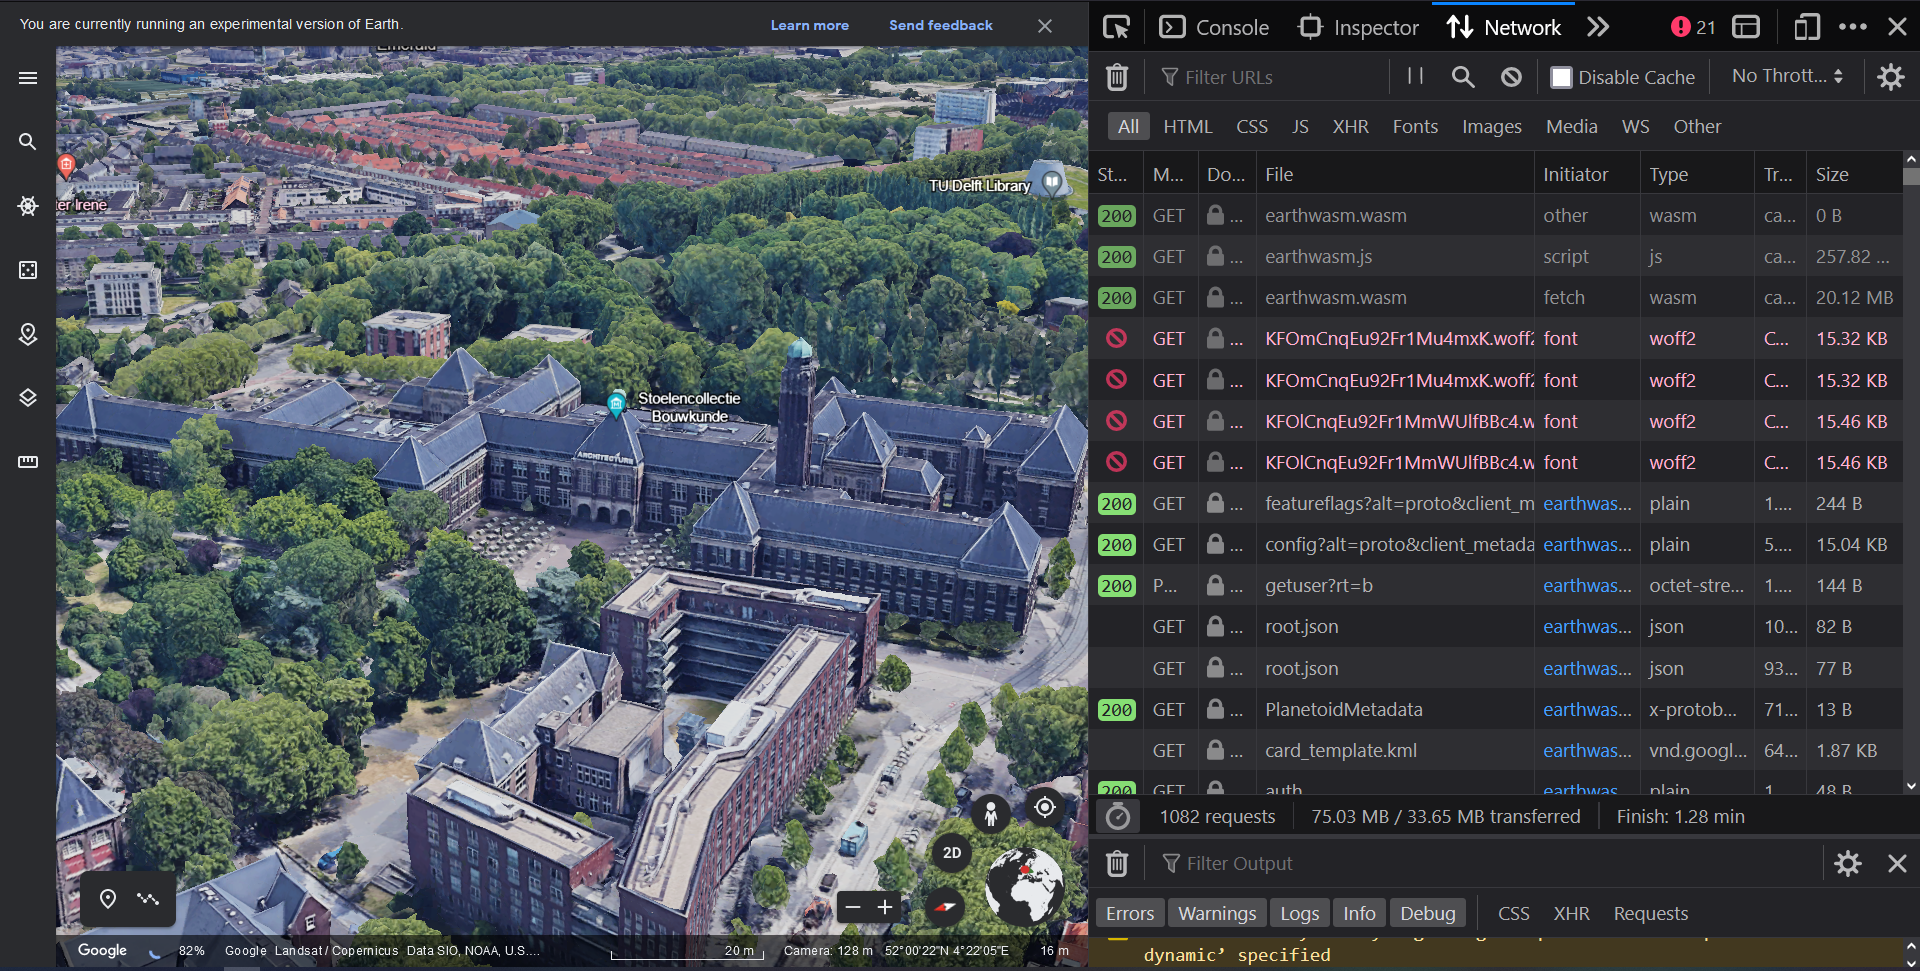
\includegraphics[width=\textwidth]{../images/google-earth-uses-webassembly.PNG}
    \caption{Google Earth utilizing WebAssembly. Source: \cite{google_google_2020}}
    \label{fig:google-earth}
  \end{minipage}
\end{figure}



The performance benefits of using WebAssembly for other purposes than geoprocessing have seen prior study. \cite{jangda_not_2019}.



% ORIGINAL PAPER

% ### x.x.x Bringing the Web up to Speed with WebAssembly
% This is the original paper introducing WebAssembly in 2017, co-written by software engineers from the major browser vendors Mozilla, Google, Apple and Microsoft. 
% It defines that a low-level compilation target should be
% save, fast, portable and compact.
% It continues by showing how previous attempts at low-level code on the web fail in at least one of these criteria, and that WebAssembly is the first to delivers on all of them. 
% The chapters following this up cover the design details of the language, and the decisions which had to be made to live up to the four criteria. 
% These details will become relevant when reasoning about why WebAssembly might be faster in one case versus another.
% <!-- proof of memory savety, proof of soundness  -->

% <!-- EXPLORE TYPES & EFFICIENT LOADING OF DATA TYPES BETWEEN UNRELATED LIBRARIES -->

% Chapter 6 and 7 also require special attention.
% Chapter 6 shows the possibilities available to a host environment for compiling, instantiating and invoking wasm binaries. 


% Chapter 7 : Implementation: 
% - validate
% - execution time
% - binary size 

% Initial benchmarks look promising
% large portion of benchmarks within 10% 

% <!-- 
% Interoperability It is possible to link multiple modules that
% have been created by different producers. However, as a low-
% level language, WebAssembly does not provide any built-in
% object model. It is up to producers to map their data types
% to numbers or the memory. This design provides maximum
% flexibility to producers, and unlike previous VMs, does not
% privilege any specific programming or object model while
% penalizing others. Though WebAssembly has a program-
% ming language shape, it is an abstraction over hardware, not
% over a programming language.
% Interested producers can define common ABIs on top of
% WebAssembly such that modules can interoperate in hetero-
% geneous applications. This separation of concerns is vital for
% making WebAssembly universal as a code format -->

%%%%%%%%%%%%%%%%%%%%%%%%%%%%%%%%%%%%%%%%%%%%%%%%%%%%%%%%%%%%%%%%%%%%%%%%%%%%%%%

% Not So Fast WebAssembly Paper 

% Paper exploring performance of WebAssembly more thorough.

% Starts out positive: current benchmarks (2019) are even better than those of the original paper (2017). 

% BUT 

% Those original papers cover a type of benchmark which uses mainly scientific operations as benchmarks. 
% Each of these operations are roughly 100 lines of code.
% This paper created a way to compile full, large-scale applications into WebAssembly, and proceeds to benchmark them. 
% They found that these types of applications run significantly slower and spikier.

% BUT 

% This might not be a problem for the scope of this research. 
% This research will deal with the originally criticized scientific purposes anyway.
% If it does turn out that wasm performs significantly slower the larger the binaries are, This research might explore disecting the C++ libraries into a number of tiny wasm Binaries, one per function for example, or per .cpp file. 
% As stated in the Wasm paper (SOURCE), it is possible to inject precompiled wasm binaries within other wasm binaries. 
% This way, the functionalities of one library could be lazy-initialized, so only the parts that are necessairy are being compiled and used. 
% Food for thought...

% ...

% A telling example of the cause of the loss in speed is this: 

% NATIVE: 
% C --{CLANG}-> x86-64 code

% WEB
% C --{EMSC}-> WASM --{JIT}-> x86-64 code 

% + Chapter 6 is very significant

% <!-- 6.4 Discussion
% It is worth asking if the performance issues identified here
% are fundamental. We believe that two of the identified is-
% sues are not: that is, they could be ameliorated by improved
% implementations. WebAssembly implementations today use
% register allocators (§6.1.2) and code generators (§6.2.1) that
% perform worse than Clang’s counterparts. However, an offline
% compiler like Clang can spend considerably more time to
% generate better code, whereas WebAssembly compilers must
% be fast enough to run online. Therefore, solutions adopted
% by other JITs, such as further optimizing hot code, are likely
% applicable here [19, 32].
% The four other issues that we have identified appear to
% USENIX Association 2019 USENIX Annual Technical Conference    117
% arise from the design constraints of WebAssembly: the stack
% overflow checks (§6.2.2), indirect call checks (§6.2.3), and
% reserved registers (§6.1.1) have a runtime cost and lead to in-
% creased code size (§6.3). Unfortunately, these checks are nec-
% essary for WebAssembly’s safety guarantees. A redesigned
% WebAssembly, with richer types for memory and function
% pointers [23], might be able to perform some of these checks
% at compile time, but that could complicate the implementa-
% tion of compilers that produce WebAssembly. Finally, a Web-
% Assembly implementation in a browser must interoperate with
% a high-performance JavaScript implementation, which may
% impose its own constraints. For example, current JavaScript
% implementations reserve a few registers for their own use,
% which increases register pressure on WebAssembly. -->

% <!-- 
% WHY PERFORMANCE LOST: LOST IN TRANSLATION 

% NATIVE: 
% C --{CLANG}-> x86-64 code

% WEB
% C --{EMSC}-> WASM --{JIT}-> x86-64 code 

% Seems to be

%  -->


% <!-- 

% TODO
% look into the specifics of the benchmarks provided 
% PolyBenchC seems to contain a lot of geometry operatinos, which seems good news for us



% SIGNIFICANT FOR GEOMATICS: 
% sync I/O is hard to do with webassembly. This could be detremental for many geomatics applciations



% The standard approach to running these applications today
% is to use Emscripten, a toolchain for compiling C and C++ to
% WebAssembly [39]. Unfortunately, Emscripten only supports
% the most trivial system calls and does not scale up to large-
% scale applications. For example, to enable applications to use
% synchronous I/O, the default Emscripten MEMFS filesystem
% loads the entire filesystem image into memory before the
% program begins executing. For SPEC, these files are too large
% to fit into memory

%  -->






\subsection{On client-side geoprocessing}

Client-side, browser based geoprocessing has seen academic interested throughout the last decade. 

- 

- timely nature

- performance 


% ### x.x.x 2014 Client-side versus Server-side Geoprocessing ...

% *These results demonstrated that the current implementation of web browsers are limited in their ability to execute JavaScript geoprocessing and not yet prepared to process data sizes larger than about 7,000 to 10,000 vertices before either prompting an unresponsive script warning in the browser or potentially losing the interest of the user.*

% This paper is very similar to what i'm doing, and it makes a conclusion that scared me at first glance. Then I saw that this is a paper out of 2014.

% The results of this paper are insightful, but do not directly applicable to this paper because of three reasons: 
% 1. The paper used javascript-based geoprocessing, not `asm.js` optimized. This is known to be inefficient. 
% 2. The paper stems from 2014. is before an incredible industry-wide performance increase of javascript interpreters. 
%    This is the result of technological development in the form of an arms race between the major browswer vendors. 
% 3. This paper will introduce WebAssembly to speed things up. 


%%%%%%%%%%%%%%%%%%%%%%%%%%%%%%%%%%%%%%%%%%%%%%%%%%%%%%%%%%%%%%%%%%%%%%%%%%%%%%%


% ### x.x.x Hybrid Geoprocessing Web Services

% This paper proposes a hybrid strategy, using the OGC Web Processing services as a starting point, and building client-side tools around it. This is different from the approach offered by this study, which starts from the well-known CGAL and GDAL geoprocessing libraries. The environment proposed by this thesis might offer OGC Web Processing services, inspired by this paper. 


%%%%%%%%%%%%%%%%%%%%%%%%%%%%%%%%%%%%%%%%%%%%%%%%%%%%%%%%%%%%%%%%%%%%%%%%%%%%%%%


% ### x.x.x Analysis of server-side and client-side Web-GIS data processing methods on the example of JTS and JSTS using open data from OSM and geoportal

% <!-- The last decade has seen a rapid evolution of processing, analysis and visualization of freely available geographic data using Open Source Web-GIS. In the beginning, Web-based Geographic Information Systems employed a thick-client approach which required installation of platform-specific browser plugins. Later on, research focus shifted to platform-independent thin client solutions in which data processing and analysis was performed by the server machine. More recently, however, the rapid development of computer hardware as well as software technologies such has HTML5 has enabled the creation of platform-independent thick clients which offer advanced GIS functionalities such as geoprocessing. This article aims to analyse the current state of Open Source technologies and publicly available geographic data sources in the context of creating cost-effective Web-GIS applications for integration and processing of spatial data. For this purpose the article discusses the availability and potential of Web-GIS architectures, software libraries and data sources. The analysis of freely available data sources includes a discussion of the quality and accuracy of crowd-sourced as well as public sector data, while the investigation of software libraries and architectures involves a comparison of server-side and client-side data processing performance under a set of real-world scenarios. The article concludes with a discussion of the choice of cost-effective Web-GIS architectures, software libraries and data sources in the context of the institution and environment of system deployment. -->

% This is a very relevant source




\subsection{On geoprocessing interfaces}

Finally, this proposal wishes to examine the state of the art of studies regarding geoprocessing interfaces. Unfortunately, most studies concerned specifically with geodata processing interfaces have a one to one relationship between application and interface. most papers do not state general user interface principles. At the same time, general UI studies are too broad, and while insightful, the scope is too big. 

Therefore, we stay close to home, and instead base interface considerations on

topic SDI research \& geoweb

interesting links can be made between

A noteworthy paper on this topic is Van den Brink's phd titled "Geospatial Data on the Web". Van den Brink states that geodata remains useful exclusively to experts in the field, despite all efforts to improve accessibility. 
She then presents the case for opening up geodata to a wider audience and more communities: "An important set of present-day users can be called “data users”: web developers, data journalists etc. who use different kinds of data, including geospatial data, directly to create applications or visualizations that supply information to end users (citizens). In order to achieve the wide re-use of geospatial data across communities, data should be easily accessible by these data users.". She also mentions the concept of FAIR geodata. Coined by \cite{mark_d_wilkinson_fair_2016}, The FAIR principles are a collection of four well-established assessment criteria used for judging the usability of data: Findable, Accessible, Interoperable, and Reusable. 

The proposed thesis acknowledges these concerns, and proposes to extend the concept of FAIR geodata to geoprocessing as well. This thesis therefore aims to make its proposed software as Findable, Accessible, Interoperable, and Reusable as possible. 

It is for these reasons that the topic of user interface will be part of this thesis. 

UI : as Findable, Accessible, Interoperable, and Reusable as possible. 

open, cross community, base on both web, w3c standards and OGC.

for these reasons, VPL chosen, so even non-programmers



- Ravi?

Lots of research has been done on the topic of VPL's, and their advantages and disadvantages. 
(I explicitly want to name the cognitive dimentions paper, it is very good and appropriate, and contains many suggestions for future VPL's)


% WebAssembly has the potential to improve all four of those criteria for software. If an application is published on the web without login requirements, makes it so there is no difference between Findability and Accessibility. As soon as it can be found, it can be accessed. 

% Additionally, \ac{wasm} is created explicitly to make software more \textit{Interoperable} and \textit{Reusable}.
% A ac{wasm} compiled library will work the same, wherever it is run. It is a manifestation of the  
% \textit{Write once, use anywhere} paradigm, not completely unrelated to the \textit{Collect once, use multiple times} paradigm, as both aim to minimize redundancy.



%%%%%%%%%%%%%%%%%%%%%%%%%%%%%%%%%%%%%%%%%%%%%%%%%%%%%%%%%%%%%%%%%%%%%%%%%%%%%%%


To the best of the author's knowledge, no papers exist coupling VPL to geoprocessing.

Still, this is being done, evident by...


Examination of multiple VPLS:






\subsection{Conclusion}

- Time is important 
- 'missing link'



\newpage
% Define the scope, extend, and how of the study
\chapter{Methodology}
\label{chap:methodology}

This chapter elaborates upon the methodology used in this study. 
The overall structure of what elements this methodology precisely consists of is presented, and how these elements came to be. 
The chapter continues with four sections, each explaining one of these components.
But first, I wish to clarify the nature in which this study is conducted. 

\subsubsection*{Nature}
The methodology of this study can be characterized as practical as opposed to theoretical, wholistic instead of specific, and iterative compared to linear. The prior works on browser-based geocomputation and geo-vpls indicate that a strong theoretical framework for a \ac{geo-web-vpl} is in place (Source). 
But, and this is especially evident in the prior studies regarding \ac{bbg} (Source), the practical implementation of these theories were only partially successful, and limited in scope. 
This necessitates a practical, wholistic approach in response. 
And, due to the investigative nature of this study, the methodology requires to iterate upon itself, instead of following a singular, linear path. 

% ...
% % Theorie: is er maar je geloofde het niet
% % praktische implementatie om de Throerie weerleggen
% The prior works on browser-based geoprocessing indicate that a theoretical framework for browser-based geoprocessing vpl is in place. 
% But, and this is especially evident in the studies regarding client-side geoprocessing, the practical implementation of these theories

% Choices: 
% - practical > theoretical : Literature study indicates enough theoretical soundness, but lots of practical questions remaining. We wish to  immediate pick up where these studies have left, and therefore we choose the direct, practical study of designing and implementing a prototype application. 
% - wholistic > specific    : Research in one sub-domain could have been more exhaustive in one of the specific sub-studies, instead of covering the full scope it does now. However, This would have been incomplete. What we do now is cover the full pipeline of using a geocomputation library: from creation to web export, to web import, to web utilization. by doing this, we can identify issues caused in one of these
% - iterative > linear      : Given this vast scope, many questions can come up from different angles. The study has to be dynamic to adapt to these demands. 

\subsubsection*{Structure}

\begin{figure}
  \centering
  \graphicspath{ {../../assets/diagrams/} }
  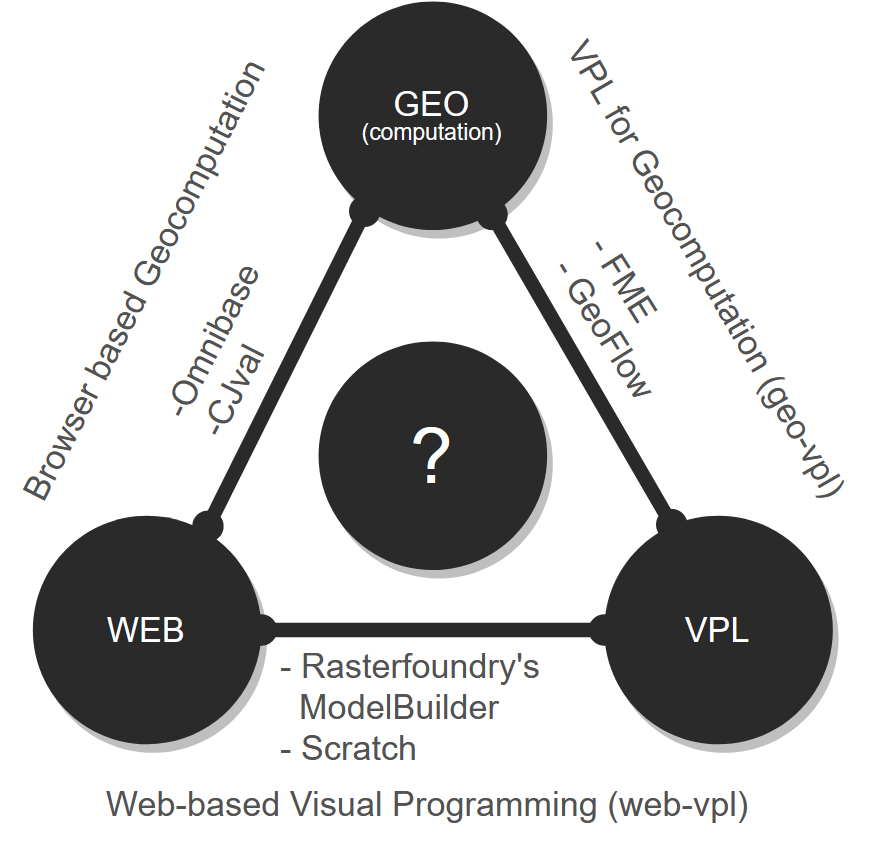
\includegraphics[width=250px]{geo-web-vpl.png}
  \caption{Triangle Model}
  \label{fig:method}
\end{figure}
  
\emph{The content of this methodology is based upon the main and supporting research questions. 
As such, it bears fruit to explain how these specific questions were chosen.}

The related studies in \refchap{chap:related} show that a \ac{geo-web-vpl} as described by this study does not exist yet. However, geo-vpls and web-vpls do exist. 
Based on this, it can be assumed that creating a visual programming environment in a web-browser must be possible. 
Using a \ac*{vpl} for geocomputation must also be possible. 

However, the absence of a geo-web-vpl indicates some sort of hinder, preventing this type of application to be realized. Either geo-VPLs were not able to be properly used in a browser, or web-based VPLs were unable to support geocomputation functionalities. 
Assuming, of course, that researchers and developers of these environments would have wanted to work towards a \ac{geo-web-vpl}.

This study starts from the second assumption: 
Apparently, web-based VPLs are unable to support existing geocomputation functionalities. 
This could be because of several reasons, of which this study identifies four major ones.

geocomputation functionalities might not be able to be properly:
\begin{itemize}[-]
  \item \textbf{compiled} into a format functional on the web
  \item \textbf{loaded} within a web-based VPL
  \item \textbf{facilitated} by the interface of a web-based VPL
  \item \textbf{used} within a web-based VPL
\end{itemize}
As it is unknown which one of these reasons ( or which combination of reasons ) is causing this barrier, the study must encompass all four of these possible hindrances, and access to what extend these aspects form a hinder towards the main goal of a \ac{geo-web-vpl}. 
Moreover, the real reason might not lie in one of these areas, but in the interplay between all of these factors. 

It is this study's objective to pose a solution to this barrier. This is stated by the main research question: \myMainRQ 

The study goes about doing so, by developing a prototype \ac{geo-web-vpl}. 
This prototype is used as an experiment and staging ground to discover the extend of possible hindrances. 
During its development, each one of these four possible hindrances has to be accounted for. 
Per hindrance, document design considerations, and run experiments, all to test to what extend this prototype \ac{geo-web-vpl} fails or succeeds to provide for this aspect. 
After this is done, we can compile a final conclusion to the main research question. 

The methodology of this study is structured to facilitate this process. 
It is subdivided into four components, each representing a sub-research question, which is in turn based upon one of these possible hindrances. The questions are posed in such a way that answering them will require us to explore the extend of the hindrance, and find possible solutions.

The remained of this chapter covers the four components of this methodology, and how this relates to this prototype. 

\begin{note}
TODO: diagram: 4 research questions -> four possible barriers of geocomputation
\end{note}

\begin{note}
TODO: diagram: show the 'locations' of the four research questions ( client / server / native, etc.)
\end{note}

%%%%%%%%%%%%%%%%%%%%%%%%%%%%%%%%%%%%%%%%%%%%%%%%%%%%%%%%%%%%%%%%%%%%%%%%%%%%%%%%%%%%%%%%%%%%%%%%%%%%%%%%%%%%%%
%%%%%%%%%%%%%%%%%%%%%%%%%%%%%%%%%%%%%%%%%%%%%%%%%%%%%%%%%%%%%%%%%%%%%%%%%%%%%%%%%%%%%%%%%%%%%%%%%%%%%%%%%%%%%%
%%%%%%%%%%%%%%%%%%%%%%%%%%%%%%%%%%%%%%%%%%%%%%%%%%%%%%%%%%%%%%%%%%%%%%%%%%%%%%%%%%%%%%%%%%%%%%%%%%%%%%%%%%%%%%
%%%%%%%%%%%%%%%%%%%%%%%%%%%%%%%%%%%%%%%%%%%%%%%%%%%%%%%%%%%%%%%%%%%%%%%%%%%%%%%%%%%%%%%%%%%%%%%%%%%%%%%%%%%%%%
%%%%%%%%%%%%%%%%%%%%%%%%%%%%%%%%%%%%%%%%%%%%%%%%%%%%%%%%%%%%%%%%%%%%%%%%%%%%%%%%%%%%%%%%%%%%%%%%%%%%%%%%%%%%%%

\section{\mySubRQOneTitle} 
\label{sec:method-one}

The first component of the methodology involved the creation of the core of the prototype application. 
Before exploring how lifting \emph{existing} geo-computation to the web might take place, this study first wished to discover to what extend the web browser is able to facilitate the interface of a 3D vpl in general, encompassed by the supporting research question : \mySubRQOne
A 3D VPL is defined as a vpl meant for generic 3D geometry processing.

The method to answer this question is defined as follows. 
The above question of \mySubRQOneTitle is further subdivided into 4 follow-up questions:
\begin{enumerate}[A]
  \item \emph{What are the requirements of a 3D VPL?}.
  \item \emph{What can be defined as 'core browser features'?}.
  \item \emph{Per requirement, to what extend can these core browser features be used to implement this requirement?}.
  \item \emph{Per implemented requirement, to what extend does this web implementation differ from existing, popular 3D VPLs?}.
\end{enumerate}

Question A and B will be answered subsequently. 
The question C is answered by \refsec{sec:app}, and the answer to the fourth question can be found in the Conclusion, as it doubles as the answer to the entire question of \mySubRQOneTitle.

\subsection*{A: 3D VPL requirements}

Based on the vpl research (SOURCE), any visual programming language must at the very least contain the following aspects: 
\begin{enumerate}[-]
  \item a visual language
  \item an interface to configure this visual language 
  \item a representation of the 'variables' and 'functions' of the visual language
  \item a way to provide input data 
  \item a way to execute the language
  \item a way to display or save output data
\end{enumerate}

Based on popular, existing 3D vpl's (Blender, Unreal, Grasshopper) A visual programming language handling 3D data should have:
\begin{enumerate}[-]
  \item A method to preview 3D data used throughout the flowchart
  \item multiple ways to determine input data (text fields, sliders) 
  \item multiple ways to view output data (text displays, 3D viewers, etc.)
\end{enumerate}

\begin{note}
  Figure out what to do with this: 
 
  A VPL should be Interactive.

    Interactivity is the defining factor of the vpl. 
    a list of standard VPL features & application features required as a base-line:  
  - Users must be able to construct a script by visual means.
  - Dataflow Modelling
  - Dragging and dropping is a ui which

  (geo-vpl features:)
  - read data from user-submitted files
  - write data to files, downloadable by the user  
  - debug / inspect data in a 3D viewer
  - draw geometry in a 3D viewer

\end{note}

\subsection*{B: Core browser features}
This study defines "Core browser features" as the set of default features implemented by the three largest browser engines. 
\begin{note}
  (show pie chart of usage statistics)
\end{note}
Based on these (FIGURE) market share statistics, the following three browsers engines appear to be the largest:
\begin{enumerate}[-]
  \item Chromium (Chrome, Edge) (Source)
  \item Gecko (Firefox) (Source)
  \item WebKit (Safari) (Source)
\end{enumerate}

The set of features common in all three browser engines are documented on (SOURCE: Mozilla). 
This includes the following set of features relevant for the 3D VPL:
\begin{enumerate}[-]
  \item WebGL (WebGL2, WebGPU)
  \item 2D Canvas API
  \item Web Workers
  \item Web Components
  \item WebAssembly
\end{enumerate}

\subsection*{C: Implementation Steps}

\begin{note}
TODO: Show the phases
\end{note}

To find the answer to question C, this study implemented the core of the prototype \ac{geo-web-vpl}.
Just like the entire study, the development trajectory for implementing will be done incrementally, ensuring results during all steps of the development. 
The first step of the phase consists of creating the basics of the \ac{gui} itself. 
A basic \ac{vpl} will be created which can only process boolean statements. 
The second step involves developing the main datamodel of the VPL, to represent the program in an object-oriented way. 
The third step adds types, geometry, and the visualization of this geometry in 3D, as well as textures / images in 2d. \
The fourth step adds geospatial data support, and adds Web Feature Services, Web Map Services, and coordinate reference systems.  

%%%%%%%%%%%%%%%%%%%%%%%%%%%%%%%%%%%%%%%%%%%%%%%%%%%%%%%%%%%%%%%%%%%%%%%%%%%%%%%%%%%%%%%%%%%%%%%%%%%%%%%%%%%%%%
%%%%%%%%%%%%%%%%%%%%%%%%%%%%%%%%%%%%%%%%%%%%%%%%%%%%%%%%%%%%%%%%%%%%%%%%%%%%%%%%%%%%%%%%%%%%%%%%%%%%%%%%%%%%%%
%%%%%%%%%%%%%%%%%%%%%%%%%%%%%%%%%%%%%%%%%%%%%%%%%%%%%%%%%%%%%%%%%%%%%%%%%%%%%%%%%%%%%%%%%%%%%%%%%%%%%%%%%%%%%%
%%%%%%%%%%%%%%%%%%%%%%%%%%%%%%%%%%%%%%%%%%%%%%%%%%%%%%%%%%%%%%%%%%%%%%%%%%%%%%%%%%%%%%%%%%%%%%%%%%%%%%%%%%%%%%
%%%%%%%%%%%%%%%%%%%%%%%%%%%%%%%%%%%%%%%%%%%%%%%%%%%%%%%%%%%%%%%%%%%%%%%%%%%%%%%%%%%%%%%%%%%%%%%%%%%%%%%%%%%%%%

\section{\mySubRQTwoTitle} 
\label{sec:method-two}
The second component of the methodology seeks an answer to the question of \mySubRQTwoTitle: \mySubRQTwo


\subsection*{Why}

Making sure a \ac{geo-web-vpl} is able to make use of native, non-js libraries is a key component, since it will mean access to powerful, industry standard geocomputation libraries like CGAL and GDAL. 
The most viable option for using a non-js library in a web browser, is by compiling it to WebAssembly \cite{haas_bringing_2017}.
Other options exist, like simply compiling non-js languages to JavaScript, but these methods have significant drawbacks \cite{haas_bringing_2017,jangda_not_2019}.
However, as described in \refsec{sec:bbg} compiling libraries to \ac{wasm} also may pose challenges:

% The study starts out with the assumption that WebAssembly must be utilized to properly compile and run existing geoprocessing libraries in a browser. This might not be as easy as using normal compilers, based on the experience gained by preliminary work (See \autoref{sec:preliminary-wasm}). WebAssembly is containerized and makes no assumptions about its source language \cite{haas_bringing_2017}, making aspects such as an SDK, sub-dependencies called using environment variables, and IO (file reading and writing) possible obstacles. 

\begin{enumerate}[-]
  \item \ac{wasm} promises a 'near native performance' (Source: Wasm). However, this can be quite situational, as multiple studies have shown \cite{jangda_not_2019} (Source: the bachelor thesis). 
  \item \ac{wasm} cannot compile all code. Its containerized nature means that code accessing a file system for example, does not work without workarounds. 
  \item Compiled \ac{wasm} code could be difficult to access and interface in a web browser. Without third-party tools, functions exposed by \ac{wasm} can only accept primitive data types as input. There is no \m{string} data type, let alone a \m{struct} or \m{object} type. 
  \item Compiling an \emph{library} to \ac{wasm} is seriously different from compiling a full \emph{application} to wasm. A library requires more complicated wasm-javascript interoperability, which third-party tools may or may not be able to provide.
\end{enumerate}
Discovering the extend and relevance of these compilation challenges for geo-computation libraries is why the sub-question of \mySubRQTwoTitle \space was included in this study. 

\subsection*{How}

% To what extend can existing geo-computation libraries be compiled for web consumption?
Two experiments are conduced to answer this supporting research question. 
The first focusses on making a clear, measurable comparison between compilation methods, where the second experiment focusses on compilation in a practical, realistic scenario. 

Both studies limit themselves to native libraries written in C++ and Rust. 
C++ was chosen, since almost all relevant geocomputation libraries are written in C++, like CGAL and PROJ. 
Rust was chosen, since this language is likely to be a future choice for geocomputation libraries, and possesses powerful WebAssembly support. 

%%%%%%%%%%%%%%%%%%%%%%%%%%%%%%%%%%%%%%%%%%%%%%%%%%%%%%%%%%%%%%%%%%%%%%%%%%%%%%%

\subsection{First Experiment}
The first experiment compares three different methods of bringing the same geocomputation procedure to the web. 
This way, quantitative, measurable aspects of these methods can be compared. 
The following three methods are tested:
\begin{enumerate}[-]
  \item Write the procedure in normal javascript
  \item Write the procedure in C++, compile to wasm using the \m{emscriptem} toolkit (Source)
  \item Write the procedure in Rust, compile to wasm using the \m{wasm-bindgen} toolkit (Source)
\end{enumerate}
These procedures are all tested within the same web application, using the same data. 
By taking two different languages, we can distinguish between shortcomings of \ac{wasm} itself, and the \ac{wasm} support of a language.  

The procedure chosen is a 2D convex hull calculation of a set of sample points. 
The chosen procedure must be small enough to clearly reason about performance differences, and yet large enough to pose a substantial computational challenge, validating the usage of \ac{wasm}.

\begin{note}
  Expand upon the procedure
\end{note}

The three methods will be compared in terms of:
\begin{enumerate}[-]
  \item performance
  \item load times
  \item memory usage
\end{enumerate}

\begin{note}
  - todo: turn features around into assessment criteria
  - performance: load times, run times
  - current state of webassembly & js. how much faster is it? is it even faster? 
     - data translation steps, do they mitigate performance gains? 
     - also given the fact that we are doing 'functions on sets'/ declarative instead of imperative styles, forced by the format of dataflow programming. 
\end{note}

The studies on browser-based geocomputation (\refsec{sec:bbg}) appear to have conducted a similar experiment, by comparing the same procedure written in C++ and javascript. 
However, these studies compared javascript against a native, non-web compilation of C++. 
This experiment also differs in distinguishing between \ac{wasm} itself, and a language's \ac{wasm} support.

%%%%%%%%%%%%%%%%%%%%%%%%%%%%%%%%%%%%%%%%%%%%%%%%%%%%%%%%%%%%%%%%%%%%%%%%%%%%%%%

\subsection{Second Experiment}
The second experiment is a qualitative comparison between compiling a full-scale library written in Rust, to a full library written in C++. 
This way, the tooling and workflow can be compared for a realistic use-case. 
The study will be conducted by attempting to compile both libraries using their respective \ac{wasm} toolsets, and noting the differences in workflow, supported features, and the resulting wasm library. 

we wish to compile these languages without 'disturbing' them: they must be kept the exact same for normal, native usage. 
We will instead create 'wrapper' libraries. 

\subsubsection*{Library One: CGAL}
The first library tested is CGAL, written in C++, compiled using \m{emscriptem}.
CGAL will be used as an exemplary C++ library. 
For one, this library is well established and very relevant to geoprocessing as a whole. 
Many other C++ geo-libraries depend on it.
Moreover, it is a sizable and complex project, making it highly likely the problems described by related works will be encountered. 
We could choose more simple libraries, but this will not be representative of most C++ geoprocessing libraries. 

\subsubsection*{Library Two: Startin}
The second library tested is the Startin library, written in Rust, compiled using \m{wasm-bindgen}.  
This library is both smaller in scope, and less well-known than CGAL. 
Ideally, a library with a size and popularity comparable to CGAL should have been chosen.
However, Rust is still a relatively unknown language in the field of GIS. 
Startin was chosen, for the triangulation functionalities it provides are comparable to that of CGAL, in terms of performance, and geometric robustness (Source). 

%%%%%%%%%%%%%%%%%%%%%%%%%%%%%%%%%%%%%%%%%%%%%%%%%%%%%%%%%%%%%%%%%%%%%%%%%%%%%%%

\section{\mySubRQThreeTitle} 
\label{sec:method-three}
In this third component of the methodology, we wish to discover how the web-exposed geocomputation libraries of \refsec{sec:method-two} can be utilized within the 3D VPL of \refsec{sec:method-one}. 
This is once more a crucial aspect for the success of the entire \ac*{geo-web-vpl}, 
and captured by the research question: \mySubRQThree

% to what extend can a web-consumable library be loaded into a web-vpl without explicit configuration?

\subsection{Why}

\begin{note}
Figure X: [geolib] --C++/Rust-> [wrapped geolib exposed to web] --wasm-> [web library wrapped for vpl] --js-> [vpl]
\end{note}

Most of the 3D vpls mentioned in the related works which offer a plugin system, or a way to load external libraries.
This way, the functionalities of the environments can be expanded upon.
However, all of these plugin / library systems require explicit 'wrapper' libraries, to explain how the functionalities a \emph{text-based} programming library map to components used in a \emph{visual} manner.
This forms a problem for the case of a \ac{geo-web-vpl} using non-js libraries. 
It would mean any non-js library would have to be wrapped twice: 
Once to expose the native library to the web (see \refsec{sec:method-two}),
And once more to map the web library to the visual language. 
While this is a possibility, in practice, two layers of indirection are not acceptable in terms of a development workflow.
This would be cumbersome, prone to errors, and hurting version control by having to synchronize between 4 software projects (See Figure X). 

This is why this third component of the methodology is focused on mitigating the need for the second wrapper library. 

\subsection{How}
For this component of the methodology, the following plan was used: 
\begin{enumerate}[-]
  \item design a library load model for the prototype \ac*{geo-web-vpl}
  \item build this library load model 
  \item assess to what extend it mitigates the need for explicit configuration
\end{enumerate}

The design is given subsequently, the build implementation and assessment can be found in \refsec{sec:impl-plugin}.

\subsection{Design \& Method}

\begin{figure}
  \centering
  \graphicspath{ {../../assets/diagrams/} }
  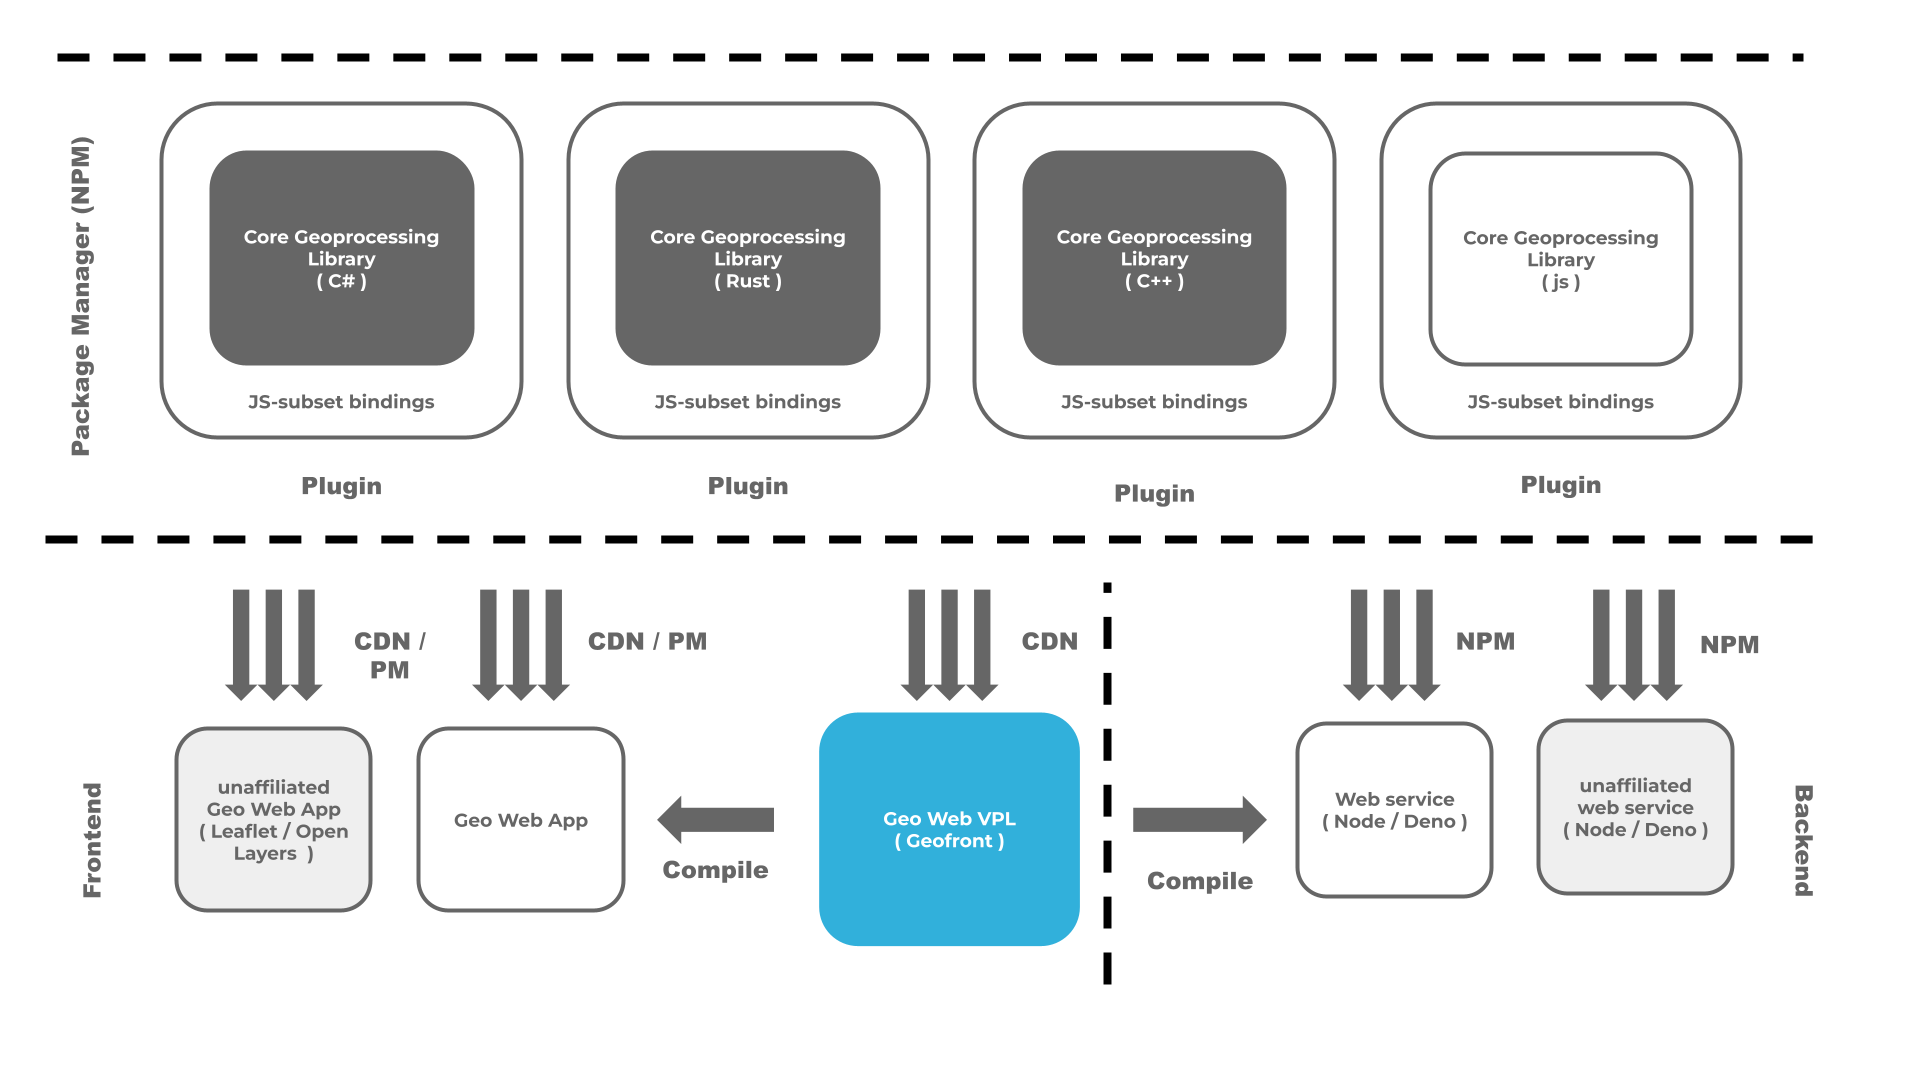
\includegraphics[width=340px]{Model Proposal.png}
  \caption{Plugin Model}
  \label{fig:method}
\end{figure}

The library model consists of two components: the design for a geo-web-vpl library, and the design for a 
loader on the side of the VPL. 
The central idea for this model is to take the wasm-wrappers created in \refsec{sec:method-two}, and to either interpret the required information from the wasm binary and related files, or, if that is impossible, add the required information in the wasm wrapper library itself.
By doing so, we make sure that at the very least, only one wrapper library is required for exposing any non-js library to the \ac{geo-web-vpl}.
The following information is required for the VPL to load a geocomputation library, and convert it into visual components:

Mandatory: 
\begin{enumerate}[-]
  \item A list of all functions present in the library, named.
  \item A list of all custom types (structs / classes) present in the library, also named.
  \item Per function:  
  \subitem A list of all input parameters, name and type.
  \subitem An output type.
\end{enumerate}

Optional: 
\begin{enumerate}[-]
  \item Per function:
  \subitem A custom name.
  \subitem A description to explain usage.

  \item Per type:
  \subitem A custom name.
  \subitem A description to explain usage.
  \subitem A definition of how to serialize and deserialize this type  
  \subitem A definition of how to render this type in 3D
  \subitem A definition of how to convert this type to basic types present within the geo-web-vpl.  
\end{enumerate}

The necessity to automate loading geocomputation libraries means that the \ac{geo-web-vpl} needs to be able to extract this information automatically. 
For scope reasons, the study limits itself to only interpret the \textbf{mandatory} information fully automatically. 
This can be achieved by using the Rust-wasm toolset "\m{wasm-bindgen}". 
\m{wasm-bindgen} is able to generate javascript wrapper bindings for a \ac{wasm} library, accompanied by TypeScript type definitions (Source). 
These are given in a 'd.ts' file, which can be understood as a header file, exposing the types required by all functions found in its corresponding javascript file. 
By including the typescript compiler in the \ac{geo-web-vpl} prototype, this header file can be loaded and interpreted to find all mandatory data, including the names and path of functions and types. 
These can then be accessed by reflecting these names and paths with the javascript files, which in turn calls the underlying \ac{wasm} binary.

The \textbf{optional} data is exposed by using 'magic methods', a strategy influenced by the python programming language (source). 
The library loader of the VPL will load certain functions, types, and methods in a special way, indicated by a naming convention. 
These functions are loaded by the vpl, but will not be converted into visual components. 
Instead, these functions are programmatically called when the VPL engine or the user requires this optional aspect. 

%%%%%%%%%%%%%%%%%%%%%%%%%%%%%%%%%%%%%%%%%%%%%%%%%%%%%%%%%%%%%%%%%%%%%%%%%%%%%%%
%%%%%%%%%%%%%%%%%%%%%%%%%%%%%%%%%%%%%%%%%%%%%%%%%%%%%%%%%%%%%%%%%%%%%%%%%%%%%%%
%%%%%%%%%%%%%%%%%%%%%%%%%%%%%%%%%%%%%%%%%%%%%%%%%%%%%%%%%%%%%%%%%%%%%%%%%%%%%%%
%%%%%%%%%%%%%%%%%%%%%%%%%%%%%%%%%%%%%%%%%%%%%%%%%%%%%%%%%%%%%%%%%%%%%%%%%%%%%%%
%%%%%%%%%%%%%%%%%%%%%%%%%%%%%%%%%%%%%%%%%%%%%%%%%%%%%%%%%%%%%%%%%%%%%%%%%%%%%%%

\section{\mySubRQFourTitle} 
\label{sec:method-four}

The final component of the methodology is dedicated to overcoming the fourth and final challenge to realizing a \ac{geo-web-vpl}, and involves the utilization of all aforementioned components. 
In this section, we wish to discover the practical usefulness of a \ac{geo-web-vpl}, encompassed by the research question : \mySubRQFour

% What are the advantages and disadvantages of using an existing geoprocessing library through a geo-web-vpl, as opposed to native utilization of said library?

\subsection{Why}
This component of the methodology is included in the study because of the following: 
It might be the case that a geo-web-vpl \emph{is} able to be interfaced using a web-browser, and \emph{is} able to load and run functions from native, non-js geo-computation libraries. 
And still, it might not be able to successfully \emph{use} these libraries. 
The entire idea of a vpl might not be sensible for the operation at hand, or some other, unforeseen aspects mitigates the practical usefulness of the environment. 
It is therefore vital to access the actual usage of the application for accessing a geocomputation library.

\subsection{How}
To answer the question of \mySubRQFourTitle, the following plan was used: 
\begin{enumerate}[-]
  \item Develop a representative use-case application within the prototype \ac{geo-web-vpl}.
  \item Develop a command line application capable of the very same process.
  \item Assess both applications according to a series of assessment questions.
\end{enumerate}

The execution of this component of the methodology is found in \refchap{chap:experiments}.

\subsection{use-case application}
The application used in both test cases is an "isocurves from DTM" process. 
But also: we want the iso-curves of a specific location. How to get this data is part of the exercise

\begin{note}
- This is subject to change, according to how much I can accomplish 

- find the required height data as WFS / WMS
- determine a boundary
- load a dtm as a regular png / tiff image
- specify the parameters, like height delta, smoothness.
- marching squares
- post-process curves
- save as wkt, geojson, or some other well-known vector format


\end{note}

\subsection{Assessment Criteria}

\begin{note}
Just ideas:

  - how to get the data you need? 
  - how to extract the part that you need?
  - how to specify the input data to the application? 
  - how to get the height parameter 'just right'? 
  
It is not about the application, is it about DOING the desired geocomputation.  

NOTE: you might want to connect this to the 3.2.1 experiment.

\end{note}
  


\newpage


\section{Preliminary Results}
\label{sec:preliminary}

As visualized in \reffig{fig:method}, two steps of this proposed methodology has already been carried out: A small-scale wasm application, and the basics of a browser-based visual programming language. These where both part of the preliminary work done in preparation of this thesis proposal. This chapter will elaborate upon these works.


\subsection{Wasm Application}
\label{sec:preliminary-wasm}

WebAssembly is a major component of this proposed thesis. However, the compilation target is still widely regarded as being "bleeding edge" \cite{jangda_not_2019}. This makes it all the more vital to gain some level of experience using the compile target before using it in more complicated scenario's. 

The Geomatics curriculum this thesis proposal is part of, offers a subject called "Research Assignment". This course offers students the opportunity to gain experience in a geomatics-related topic of choice, and this made it the perfect context to try out WebAssembly for a geomatics web application.

The assignment given was to deliver a prototype for an online cityJSON validator. 
WebAssembly was to be used to perform a very fast JSON schema check over a user submitted json, among other things. 
This assignment was carried out successfully, and the delivered prototype (\reffig{fig:cjval-prototype}) played a role in the official CityJSON validator (\reffig{fig:cjval-official}), which uses WebAssembly. 

\begin{figure}[!tbp]
    \centering
    \begin{minipage}[b]{0.45\textwidth}
      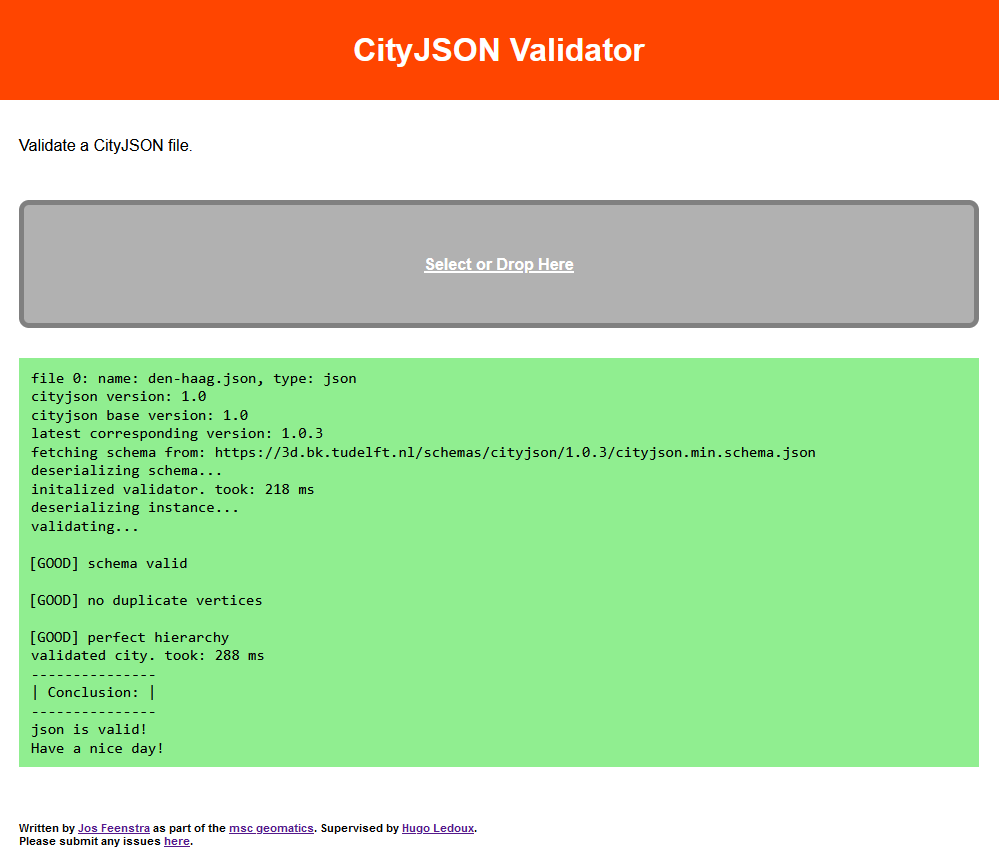
\includegraphics[width=\textwidth]{../images/cjval-prototype.PNG}
      \caption{The prototype}
      \label{fig:cjval-prototype}
    \end{minipage}
    \hfill
    \begin{minipage}[b]{0.45\textwidth}
      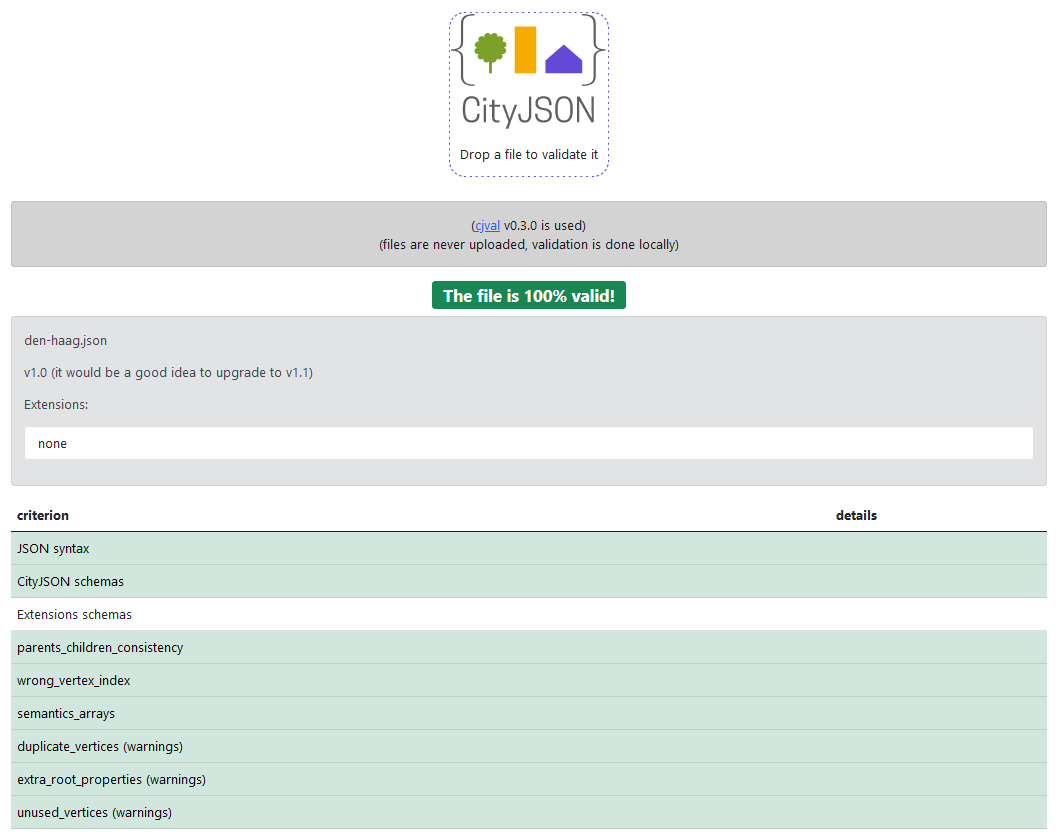
\includegraphics[width=\textwidth]{../images/cjval-official.PNG}
      \caption{The official validator}
      \label{fig:cjval-official}
    \end{minipage}
\end{figure}

Creating this application offered many key insights of working with WebAssembly, which will undoubtedly play an important role in the proposed thesis. 

% The question of what a FAIR geoprocessing interface should look like, together with partially implementing this interface, was the topic of a second preliminary study. 
% As state before, this question's scope it wide, the question is difficult to proof, and can be considered slightly off-topic. We will therefore start from the presupposition that a web-based \ac{vpl} is a FAIR geoprocessing interface. This presupposition is informed by the following reasons: 

% \begin{itemize}
%   \item A \ac{vpl} can be seen as a compromise between a programming language and a full \ac{gui}. This has the advantage of serving both geodata experts, as well as the "data user" group depicted by \cite{brink_geospatial_2018}. The latter group might not be prepared to code, but would like to chain together geodata processing functions.
%   \item \ac{vpl}'s have a clear advantage when dealing with data containing a visual component. Making in-between steps graphically debugable is very difficult to do with regular programming languages. Even programmers often use \ac{vpl}'s when programming shaders, for instance (SOURCE). 
%   \item Geodata processing experts often depict geodata pipelines as a flowchart, graph, or a literal pipeline. 
% \end{itemize}

% Additionally, using a \ac{vpl} for geodata processing is not uncommon. examples of applications like these are FME, (SOURCE), QGIS's Model Builder (SOURCE), and Geoflow (SOURCE). Applications concerned with geometry manipulation in general also often choose \ac{vpl}'s, like Houdini(SOURCE), Blender's Geometry Nodes(SOURCE), and Rhino's Grasshopper(Source).


% \subsubsection*{Design}

% The way this \ac{vpl} was designed was influenced by the FAIR principles \cite{mark_d_wilkinson_fair_2016}, the analysis of exiting geo-vpl's mentioned above, as well as by and studies discussing the usability aspects of VPL's \cite{green_usability_1996, peters_geoflow_2019}. We present a MOSCOW analysis of the requirements of this environment: 

% Must Have
% \begin{itemize}
%   \item Users must be able to configure their own graphs / flowchart. This involves \ac{ui} features like placing operations and drawing relationships between them. 
%   \item This flowchart must be able to compute itself. This can be realized by using a \ac{dag}.
% \end{itemize}

% Should Have
% \begin{itemize}
%   \item The environment should support operations users have come to expect from applications in general, 
%   like copy, paste, save, load, undo, redo, etc. 
%   \item the environment should support GIS operations such as WFS, WMS, and CRS translations.
%   \item The environment should support GIS input actions such as selecting coordinates on a map.  
%   \item Created scripts should be able to run without the \ac{gui}. It would even be better to be able to compile the environment to plain JavaScript. 
%   \item Created scripts should be sharable online by means of a link. This can be realized by either storing scripts on a server, or by saving to and loading scripts from a hash which can be included in a link. 
%   \item Despite the goal of becoming a geoprocessing environment, we should enable the tool to additionally be used for acquiring, visualizing, and saving geodata.
 
% \end{itemize}

% Could Have
% \begin{itemize}
%   \item The environment could eventually be used completely offline again, like a normal, installable application, or a vscode plugin. Tools like 'electron' support this. 
%   \item The environment could eventually support many input and output data formats, like cityJSON, .obj, and GLTF. 

% \end{itemize}

% Won't Have
% \begin{itemize}
%   \item The environment will not include a full IDE.
%   \item The environment will not have login functionalities. The flowcharts will not be saved on a server.  
% \end{itemize}


\subsection{VPL Prototype}
\label{sec:preliminary-vpl}

The 'GeoFront' use case application has also received preliminary attention, in the form of a demo build. The focus of this demo was on the \ac{gui}, and as such, it supports only basic types. 

\begin{figure}[!tbp]
  \centering
  \begin{minipage}[b]{1.0\textwidth}
    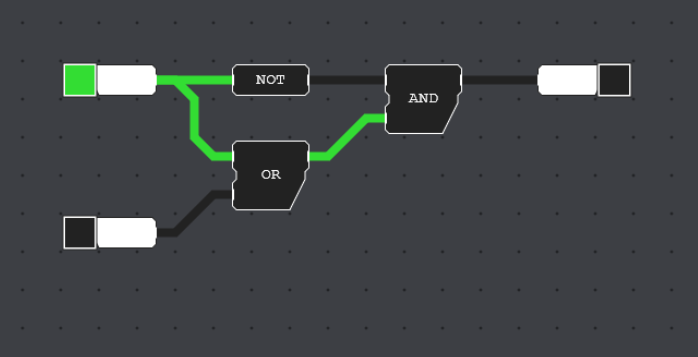
\includegraphics[width=\textwidth]{../images/geofront-1.PNG}
    \caption{The 'Geofront' environment.}
    \label{fig:geofront-1}
  \end{minipage}
\end{figure}


\begin{figure}[!tbp]
  \centering
  \begin{minipage}[b]{1.0\textwidth}
    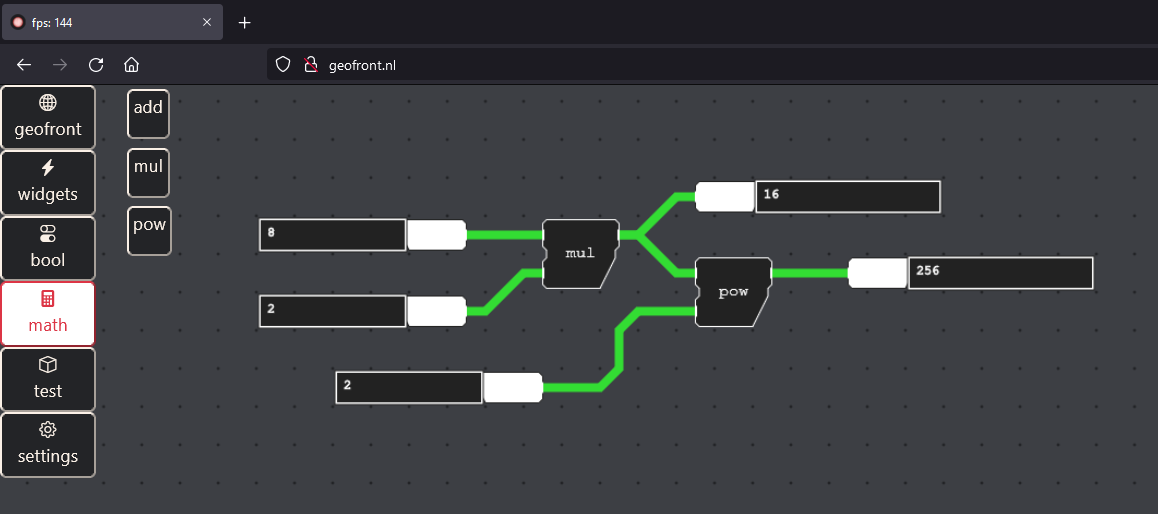
\includegraphics[width=\textwidth]{../images/geofront-2.PNG}
    \caption{GeoFront, showcasing basic mathematics.}
    \label{fig:geofront-2}
  \end{minipage}
\end{figure}


The current application looks like \reffig{fig:geofront-1}. Input, output and operators can be placed on a canvas, and lines can be drawn in between these components. The graph then determines the order of execution by means of a \ac{dag}, and executes this any time an input has altered, or when the graph has been reconfigured. All graphics are provided by using the 2d Canvas API, native to modern web browsers.

Besides boolean values and operations, basic mathematical operations are also supported (see \reffig{fig:geofront-2}). Panels utilizing html are used to provide inputs and showcase outputs. 

\reffig{fig:geofront-3} shows how a graph can be saved as JavaScript. This script can be run completely independent of the geofront application, as long as the libraries used by the individual operation are included. The script can also itself be turned into an operation. This is meant for encapsulation, just like how regular programming languages support the creation and re-use of functions.

Lastly, \reffig{fig:geofront-4} shows that the first steps are made towards structs, objects, and other complex data types. 

\begin{figure}[!tbp]
  \centering
  \begin{minipage}[b]{1.0\textwidth}
    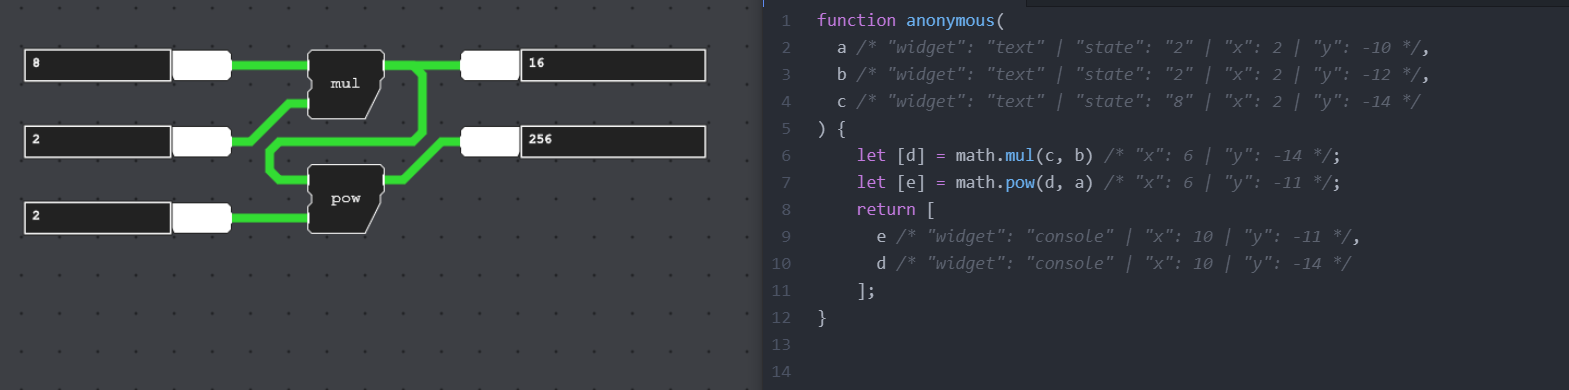
\includegraphics[width=\textwidth]{../images/geofront-3.PNG}
    \caption{GeoFront, showcasing javascript interoperability.}
    \label{fig:geofront-3}
  \end{minipage}
\end{figure}

\begin{figure}[!tbp]
  \centering
  \begin{minipage}[b]{1.0\textwidth}
    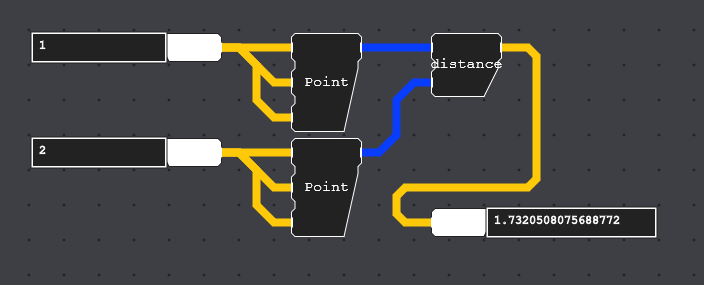
\includegraphics[width=\textwidth]{../images/geofront-4.PNG}
    \caption{GeoFront, showcasing support for basic structs. Types are color coded.}
    \label{fig:geofront-4}
  \end{minipage}
\end{figure}
\newpage
%-------------------------------------------------------------------------------------------------%
% Having a Gantt chart is probably a better idea then just a list.
\newpage
\section{Planning and Organization}

This study will be written as a MSc Geomatics Thesis. As such, several assessment dates are in order:   

\begin{itemize}
    \item The Graduation plan presentation (P2) will take place at January 28th. 
    \item The Midterm progress meeting  (P3) will take place at the end of March / beginnen of April. 
    \item The Go/no-go assessment (P4) will take place mid May.
    \item The Public presentation and final assessment (P5) will take place at the end of June.
\end{itemize}

A Gantt chart (\reffig{fig:gantt}) explains how these assessment dates relate to the overall methodology.




\afterpage{
  \begin{landscape}
  \begin{figure}
  \newganttlinktype{f-m}{
  \ganttsetstartanchor{on right=1}
  \ganttsetendanchor{on left=0}
  \draw[/pgfgantt/link]
    ([xshift=-.2pt]\xLeft, \yUpper) --       % xshift to fit arrow
    node[pos=.5, /pgfgantt/link label node] {\ganttlinklabel} 
    (\xRight, \yLower);
  }
  \newganttlinktype{rdldr*}{%
    \draw [/pgfgantt/link]
      (\xLeft, \yUpper) --
      (\xLeft + \ganttvalueof{link bulge 1} * \ganttvalueof{x unit},
        \yUpper) --
      ($(\xLeft + \ganttvalueof{link bulge 1} * \ganttvalueof{x unit},
        \yUpper)!%
        \ganttvalueof{link mid}!%
        (\xLeft + \ganttvalueof{link bulge 1} * \ganttvalueof{x unit},
        \yLower)$) --
      ($(\xRight - \ganttvalueof{link bulge 2} * \ganttvalueof{x unit},
        \yUpper)!%
        \ganttvalueof{link mid}!%
        (\xRight - \ganttvalueof{link bulge 2} * \ganttvalueof{x unit},
        \yLower)$) --
      (\xRight - \ganttvalueof{link bulge 2} * \ganttvalueof{x unit},
        \yLower) --
      (\xRight, \yLower);%
  }
  \ganttset{
    link bulge 1/.link=/pgfgantt/link bulge,
    link bulge 2/.link=/pgfgantt/link bulge}
  \definecolor{barpurple}{RGB}{195, 208, 212}
  \definecolor{grouppurple}{RGB}{150, 217, 217}
  \definecolor{progressgreen}{RGB}{255, 199, 99}
  \definecolor{groupprogress}{RGB}{110, 219, 110}
  \definecolor{linkblue}{RGB}{65,105,225}
  \setganttlinklabel{s-s}{}
  \setganttlinklabel{f-s}{}
  \setganttlinklabel{f-f}{}
  \setganttlinklabel{f-m}{}
  \sffamily

  \begin{ganttchart}[
      canvas/.append style={fill=none, draw=black!5, line width=.75pt},
      x unit=5.5mm,
      y unit chart=6.2mm,
      hgrid style/.style={draw=black!5, line width=.75pt},
      vgrid={*{30}{draw=black!5}},% line width=.75pt},
      today=4,
      today rule/.style={
        draw=black!64,
        dash pattern=on 3.5pt off 4.5pt,
        line width=1.5pt
      },
      %today label font=\small\bfseries,
      title/.style={draw=none, fill=none},
      %title label font=\bfseries\footnotesize,
      title label node/.append style={below=7pt},
      include title in canvas=false,
      %bar label font=\mdseries\small\color{black!70},
      bar label node/.append style={left=0cm},
      bar/.append style={draw=none, fill=progressgreen},
      bar incomplete/.append style={fill=barpurple},
      %bar progress label font=\mdseries\footnotesize\color{black!70},
      group/.append style={draw=none, fill=groupprogress}
      group incomplete/.append style={fill=grouppurple},
      group left shift=0,
      group right shift=0,
      group height=.5,
      group peaks tip position=0,
      group label node/.append style={left=0cm},
      link/.style={-latex, line width=1.5pt, linkblue},
      link label node/.append style={below left=-2pt and 0pt},
      link bulge=.5
    ]{1}{30}

    \gantttitle[title label node/.append style={below left=7pt and -3pt}]{WEEKS}{1}
    \gantttitlelist{2,...,25}{1} \\
    
    % Phase 1
    % \ganttnewline 
    \ganttgroup[progress=20]{Phase 1: Compile}{5}{9} \\
    \ganttbar[progress=80]{compile a small C++ geoprocessing script to wasm}{5}{6} \\
    \ganttbar[progress=0]{compile CGAL \& GDAL to wasm}{7}{9} \\
    \ganttbar[progress=0]{experiment with compilation methods}{7}{9} \\ 
    % [grid]
    
    % Phase 2
    % \ganttnewline 
    \ganttgroup[progress=20]{Phase 2: Interface}{10}{14} \\
    \ganttbar[progress=60]{Develop the basics of a browser based vpl}{10}{11} \\
    \ganttbar[progress=0]{Add basic geometry processing and visualization support}{12}{13} \\ 
    \ganttbar[progress=0]{Add auxiliary utilities}{13}{13} \\ 
    \ganttbar[progress=0]{Add WFS \& WMS inputs}{14}{14} \\ 
    % [grid]
    
    % Phase 3
    % \ganttnewline 
    \ganttgroup[progress=0]{Phase 3: Distribute}{15}{20} \\
    \ganttbar[progress=0]{Add Wasm plugin support to the VPL}{15}{15} \\ 
    \ganttbar[progress=0]{Add gdal \& cgal as plugins}{16}{17} \\
    \ganttbar[progress=0]{Experiment using different distribution strategies}{17}{20} \\
    
    % Phase 4
    % \ganttnewline 
    \ganttgroup[progress=0]{Phase 4: Utilize}{18}{20} \\
    \ganttbar[progress=0]{Create and assess an application using this environment}{18}{20}\\

    \ganttnewline 
    \ganttbar[progress=10]{Write P4 report}{4}{20}\\
    \ganttmilestone[]{P4 Assessment}{20} \ganttnewline
    \ganttmilestone[]{P5 Assessment}{25}

  \end{ganttchart}

  \caption{Gantt chart of the methodology, made with pgfgantt, Source: Author}
  \label{fig:gantt}
  \end{figure}
  \end{landscape}
}
\newpage
%-------------------------------------------------------------------------------------------------%
% Since specific data and tools have to be used, it’s good to present these concretely, 
% so that the mentors know that you have a grasp of all aspects of the project.
\newpage
\section{Tools and Data}

\subsection{Tools}
In order to perform the study proposed, several tools are needed. All tools mentioned are free and open source.

\subsubsection*{Typescript}
Typescript will be the programming language used for creating the main visual programming language application. Typescript is chosen over javascript, since the safeguards and type checks provided at compile time are very beneficial when creating medium to large scale applications. 

Depending on the size of the application, a framework such as React or Vue might be used to offer structure.

\subsubsection*{HTML5}
HTML5 provides adequate features in order to create the actual \ac{gui}. Buttons and panels can be created using just HTML. The Canvas 2d API is an excellent method of drawing 2d shapes, and can be used to draw the components and cables of the VPL itself. Alternatively, this can also be done using Scalable Vector Graphics (SVG's). 

\subsubsection*{WebGl}
WebGl allows for performant web visualizations using syntax similar to OpenGL. This will be used to make preview visualizations of 2D and 3D data. Modern web browsers are equipped with WebGl by default. 

\subsubsection*{WebAssembly}
WebAssembly binaries, and its surrounding tooling, will of course be used. Modern browsers provide WebAssembly support by default. For running WebAssembly files locally, WASI, a native WebAssembly Runtime will be utilized. 

\subsubsection*{C++ \& Emscriptem}
Most geoprocessing libraries commonly used within the geospatial community are C++ based libraries, such as CGAL \& GDAL. A toolchain called Emscripten will be used to compile these libraries into WebAssembly. Additional C++ wrapper libraries might be written if direct compilation proves to be difficult. 

\subsubsection*{Rust \& wasm-pack}
Rust is the community preference for developing programs targeting wasm. 
The rust ecosystem contains a number of powerful tools such as wasm-pack, and the standard rust compiler includes wasm as a compilation target by default. If during this study a need arises for newly written geoprocessing libraries, Rust will be preferred over C++ for these reasons. But, by default, Rust will not be used during this study, since no well-known geoprocessing libraries exist within its ecosystem.

\subsection{Data}
This study is not dependent on specific datasets. However, in order to use Geodata processing libraries, we will have need of some data to start with. Demo data of the netherlands will be used, using the WFS and WMS services provided by the Dutch geodata portal PDOK. 


% [Appendix]
\newpage

\bibliographystyle{apalike}
\bibliography{library}

% \printbibliography

\end{document}